\documentclass[
ngerman,
oneside,
 leqno, % optional, zeigt Equation Nummern auf der linken Seite
 fleqn, % optional, zeigt Equations linksbuendig an
]{book} 

\setlength{\parskip}{1em}
\setlength{\parindent}{0em}
\renewcommand{\baselinestretch}{1.15}
\renewcommand{\arraystretch}{1.0}

\include{env.tex} % env.tex is generated by build_user_manual.sh
\include{preambel}

\pagestyle{empty}
\begin{document}

\pagenumbering{gobble}


\begin{center}
	\begin{figure}[H]
		\center
		
\includegraphics[scale=0.2]{img/MOKKA-Budget-Logo}
	\end{figure}
	\textbf{MOKKA Budget} \\
	\vspace{.1cm}
	Idee und Entwicklung von Tim Poerschke \\
	\vspace{.1cm}
	Mit Unterstützung von \\ Noah Skrzypczyk \\
	\vspace{2cm}
	\textbf{\LARGE
		Benutzerhandbuch
	}\\	
	\vspace{2cm}
	Version \APPVERSION \\
	\today
\end{center}

\vfill

\url{https://github.com/tpoerschke/mokka-budget} \\
\url{https://timkodiert.de/project/mokka-budget}

\clearpage


\pagestyle{fancy}

\fancyhead[LO]{}
\fancyhead[RO]{\rightmark}
\fancyfoot[CE,CO]{\thepage}


% Gliederung römisch
\clearpage
\pagenumbering{roman}

\tableofcontents

\clearpage
\pagenumbering{arabic}

\chapter{Stamm- \& Bewegungsdaten}

Die Software unterscheidet zwischen zwei Typen von Umsätzen:

\begin{itemize}[nosep]
	\item Wiederkehrende Umsätze
	\item (Einzigartige) Umsätze
\end{itemize}

\section{Wiederkehrende Umsätze} \label{sec:fixedExpenses}

Wiederkehrende Umsätze treten in einem bestimmten Rhythmus auf (bspw. vierteljährlich oder monatlich) oder aber auch unregelmäßig -- dafür aber wiederkehrend (bspw. Tanken) -- auf.

\begin{figure}[ht!]
	\centering
	\includegraphics[width=\textwidth]{img/Screenshot-FixedExpenses-MDV}
	\vspace{-2em}
	\caption{Listen- \& Detailansicht der wiederkehrenden Umsätze}
	\label{fig:mdvFixedExpenses}
\end{figure}

In der Detailansicht (s. Abbildung \ref{fig:mdvFixedExpenses} rechts) kann u. a. der Zyklus/Rhythmus (s. "`Zahlungen"' des Umsatzes und die Importregeln festgelegt werden. Beide Angaben sind optional.

\renewcommand{\arraystretch}{1.5}
\begin{table}[!ht]
\centering
\begin{tabular}{|p{6cm}|p{8cm}|}
\hline 
\textbf{Feld} & \textbf{Beschreibung} \\ 
\hline 
Position * & Bezeichnung des Umsatzes \\ 
\hline 
Bemerkung & Anmerkung zum Umsatz \\ 
\hline 
Richtung * & Richtung (Einnahme oder Ausgabe) \\ 
\hline 
Kategorien & Kategorien, denen der Umsatz zugeordnet ist \\ 
\hline 
Zahlungen nur für die Zukunft (und den aktuellen Monat) verwenden & Wenn die Checkbox ausgewählt ist, werden die konfigurierten Zahlungen nicht für die Vergangenheit verwendet (s. Beispiel unten) \\ 
\hline 
\end{tabular} 
\caption{Konfigurationsmöglichkeiten im Tab "`Informationen"'}
\end{table}
\renewcommand{\arraystretch}{1.0}

\renewcommand{\arraystretch}{1.5}
\begin{table}[!ht]
\centering
\begin{tabular}{|p{6cm}|p{8cm}|}
\hline 
\textbf{Feld} & \textbf{Beschreibung} \\ 
\hline 
Betrag * & Höhe des Umsatzes \\ 
\hline 
Art * & Rhythmus des Umsatzes (monatlich, vierteljährlich, halbjährlich, jährlich) \\ 
\hline 
Von * & Bspw. ab wann der Umsatz in dieser Höhe ansteht \\ 
\hline 
Bis & Bspw. bis wann der Umsatz in dieser Höhe ansteht (kann leer gelassen werden, wenn der Umsatz aktuell in dieser Höhe ansteht) \\ 
\hline 
\multicolumn{2}{|p{14cm}|}{In der Tabelle können mehrere "`Zahlungen"' hinterlegt werden. Das ermöglicht die Abbildung von steigenden oder sinkenden Umsätzen, wie es bspw. bei Versicherungsbeiträgen häufig der Fall ist.} \\ 
\hline 
\end{tabular} 
\caption{Konfigurationsmöglichkeiten im Tab "`Zahlungen"'}
\end{table}
\renewcommand{\arraystretch}{1.0}

\renewcommand{\arraystretch}{1.5}
\begin{table}[!ht]
\centering
\begin{tabular}{|p{6cm}|p{8cm}|}
\hline 
\textbf{Feld} & \textbf{Beschreibung} \\ 
\hline 
Tabelle "`Importregeln"' & Diese Tabelle ermöglicht die Verwaltung einer Liste an Importregeln (s. Kapitel \ref{chap:import}) \\ 
\hline 
Tabelle "`Zugeordnete Importe"' & Listet alle zugeordneten Importe auf (readonly) \\ 
\hline 
\end{tabular} 
\caption{Konfigurationsmöglichkeiten im Tab "`Import"'}
\end{table}
\renewcommand{\arraystretch}{1.0}

\begin{infobox}
\textbf{Hinweis zu importierten Umsätzen}: Sollten zu einer Ausgabe reale Umsätze importiert worden sein, werden in den Übersichten (bspw. Monatsansicht) der Betrag dieser importierten Umsätze verwendet und der im System konfigurierte Betrag nur noch als Fallback verwendet. Eine detailliertere Beschreibung findet sich in Kapitel \ref{chap:import}. 
\end{infobox}

Da reale Ausgaben (bzw. Importe) über die Importregeln einer regelmäßigen Ausgabe zugeordnet werden können und dann dieser reale Umsatz in der Software angezeigt wird, können auch wiederkehrende Ausgaben mit schwankenden Beträgen -- wie es beim Tanken der Fall ist -- gruppiert werden.

\subsection*{Beispiel: Tanken}

Die Ausgabe "`Tanken"' soll als wiederkehrender Umsatz (Richtung "`Ausgabe`"') im System abgebildet werden. Dazu kann eine "`Zahlung"' in der Höhe von bspw. 80 Euro monatlich angelegt werden. Allerdings wird nicht jeden Monat getankt, weshalb die Checkbox "`Zahlungen nur für die Zukunft (und den aktuellen Monat) verwenden"' ausgewählt wird. Somit werden bspw. in der Analyseansicht für vergangene Monate die realen Ausgaben angezeigt -- wie sie vom Konto importiert wurden --, während für die Zukunft weiterhin die geplanten Zahlungen aufgeführt werden. Wenn man regelmäßig an einer Star- oder Aral-Tankstelle tankt und mittels Visa-Karte bezahlt, könnten zwei Importregeln konfiguriert werden, die jeweils  "`VISA STAR"' und "`VISA ARAL"' als "`Empfänger enthält"' eingetragen haben. 

Sollte das Import-Feature nicht genutzt werden, kann ein "`realer Umsatz"' auch manuell als (einzigartiger) Umsatz (bzw. Ausgabe) konfiguriert und mit der wiederkehrenden Ausgabe "`Tanken"' verknüpft werden. Dann wird für den entsprechenden Monat ebenfalls der gesamte Betrag dieser Ausgabe verwendet, statt der geplanten Zahlung der wiederkehrenden Ausgabe.


\section{(Einzigartige) Umsätze}

Einzigartige Umsätze treten einmalig oder selten auf, sodass es keinen Mehrwert bietet, diese als regelmäßige Umsätze zu gruppieren (da bspw. keine wiederkehrenden Importe zu Ausgaben dieser Art erwartet werden). Beispiele wären hier der Besuch eines Restaurants oder Ausgaben für Geschenke.

\begin{figure}[ht!]
	\centering
	\includegraphics[width=\textwidth]{img/Screenshot-UniqueExpenses-MDV}
	\vspace{-2em}
	\caption{Listen- \& Detailansicht der (einzigartigen) Umsätze}
	\label{fig:mdvFixedExpenses}
\end{figure}

In der Listenansicht werden standardmäßig nur die Umsätze angezeigt, die keinem wiederkehrenden Umsatz zugeordnet sind. Sollen Umsätze angezeigt werden, die wiederkehrenden Umsätzen zugeordnet sind -- und somit den wiederkehrenden Umsatz für den Monat überschreiben --, kann dies über das Dropdown-Menü oben rechts über der Listenansicht erreicht werden.

Die Konfigurationsmöglichkeiten im Tab "`Informationen"' sind in Tabelle \ref{tab:uniqueTurnoverInfoTab} beschrieben. Der Tab "`Positionen"' ermöglicht das hinterlegen einzelner Positionen des Umsatzes, die für sich kategorisiert werden können und ihre eigene Richtung (Einnahme oder Ausgabe) haben. Die Summe dieser Positionen ergibt den Betrag eines (einzigartigen) Umsatzes.

\renewcommand{\arraystretch}{1.5}
\begin{table}[!ht]
\centering
\begin{tabular}{|p{6cm}|p{8cm}|}
\hline 
\textbf{Feld} & \textbf{Beschreibung} \\ 
\hline 
\hline 
\multicolumn{2}{|c|}{Allgemein} \\ 
\hline 
Rechnungsteller * & Rechnungsteller (wird in anderen Ansichten als Name des Umsatzes angezeigt)  \\ 
\hline 
Datum * & Datum des Umsatzes \\ 
\hline 
Bemerkung & Optionaler Kommentar zum Umsatz \\ 
\hline 
Pfad zum Beleg / Kassenbon & Optionaler Dateipfad zum Beleg. Wird als Bild in dieser Ansicht angezeigt \\ 
\hline 
Wiederkehrender Umsatz & Optionaler wiederkehrender Umsatz. Sollte ein wiederkehrender Umsatz ausgewählt sein, wird der Betrag dieses Umsatzes für den Monat verwendet (und nicht der konfigurierte Betrag am wiederkehrenden Umsatz) \\ 
\hline 
\hline 
\multicolumn{2}{|c|}{Import (readonly)} \\ 
\hline 
Empfänger & Empfänger wie er in der Quelle (Konto) des Umsatzes aufgeführt ist \\
\hline
Verwendungszweck & Verwendungszweck wie er in der Quelle (Konto) des Umsatzes aufgeführt ist \\
\hline 
Buchungstext & Art des Umsatzes (bspw. Lastschrift oder Überweisung) wie er in der Quelle (Konto) des Umsatzes aufgeführt ist \\
\hline 
Betrag & Realer Betrag des Umsatzes wie er in der Quelle (Konto) des Umsatzes aufgeführt ist \\
\hline 
\end{tabular} 
\caption{Konfigurationsmöglichkeiten im Tab "`Informationen"'}
\label{tab:uniqueTurnoverInfoTab}
\end{table}
\renewcommand{\arraystretch}{1.0}

\begin{infobox}
\textbf{Hinweis zu importierten Umsätzen}: Für jeden importierten Umsatz wird ein (einzigartiger) Umsatz angelegt, der eventuell einem wiederkehrenden Umsatz zugeordnet ist und den dort konfigurierten Betrag für den Monat überschreibt. Da die Positionen des importieren Umsatzes im System bearbeitet werden können, kann die Summe der Positionen ungleich dem importierten Betrag sein. In dieser Situation wird eine Warnung unterhalb des importierten Betrags angezeigt, aber der konfigurierte Betrag vom System verwendet. 
\end{infobox}

\section{Kategorien und Kategoriegruppen}

Zur Kategorisierung von Umsätzen können Kategorien herangezogen werden, die nochmal zu Gruppen zusammengefasst werden können. An Kategorien kann jeweils ein Budget konfiguriert werden, welches in der Monats- uns Analyseansicht angezeigt wird. 

Die Kategoriegruppen sind aktuell nur als Datenmodell implementiert und finden innerhalb des Systems keine Anwendung in den Ansichten zur Auswertung der Umsätze.

\section{Abrechnungen}

Abrechnungen ermöglichen die Gruppierung von Umsätzen, die sich auf ein gemeinsames Ereignis beziehen. Ein Beispiel wäre eine Urlaubsreise, bei der verschiedene Ausgaben (bspw. Flug, Hotel, Mietwagen) anfallen.

Abrechnungen bestehen aus einer Bezeichnung, einem optionalen Beschreibung und einer Liste an Umsätzen. Über diese Umsätze wird eine Summe gebildet. Die Umsätze werden mittels eines Dialogs, der eine Suche über die letzten 100 Umsätze ermöglicht, zur Abrechnung hinzugefügt.

\begin{figure}[ht!]
	\centering
	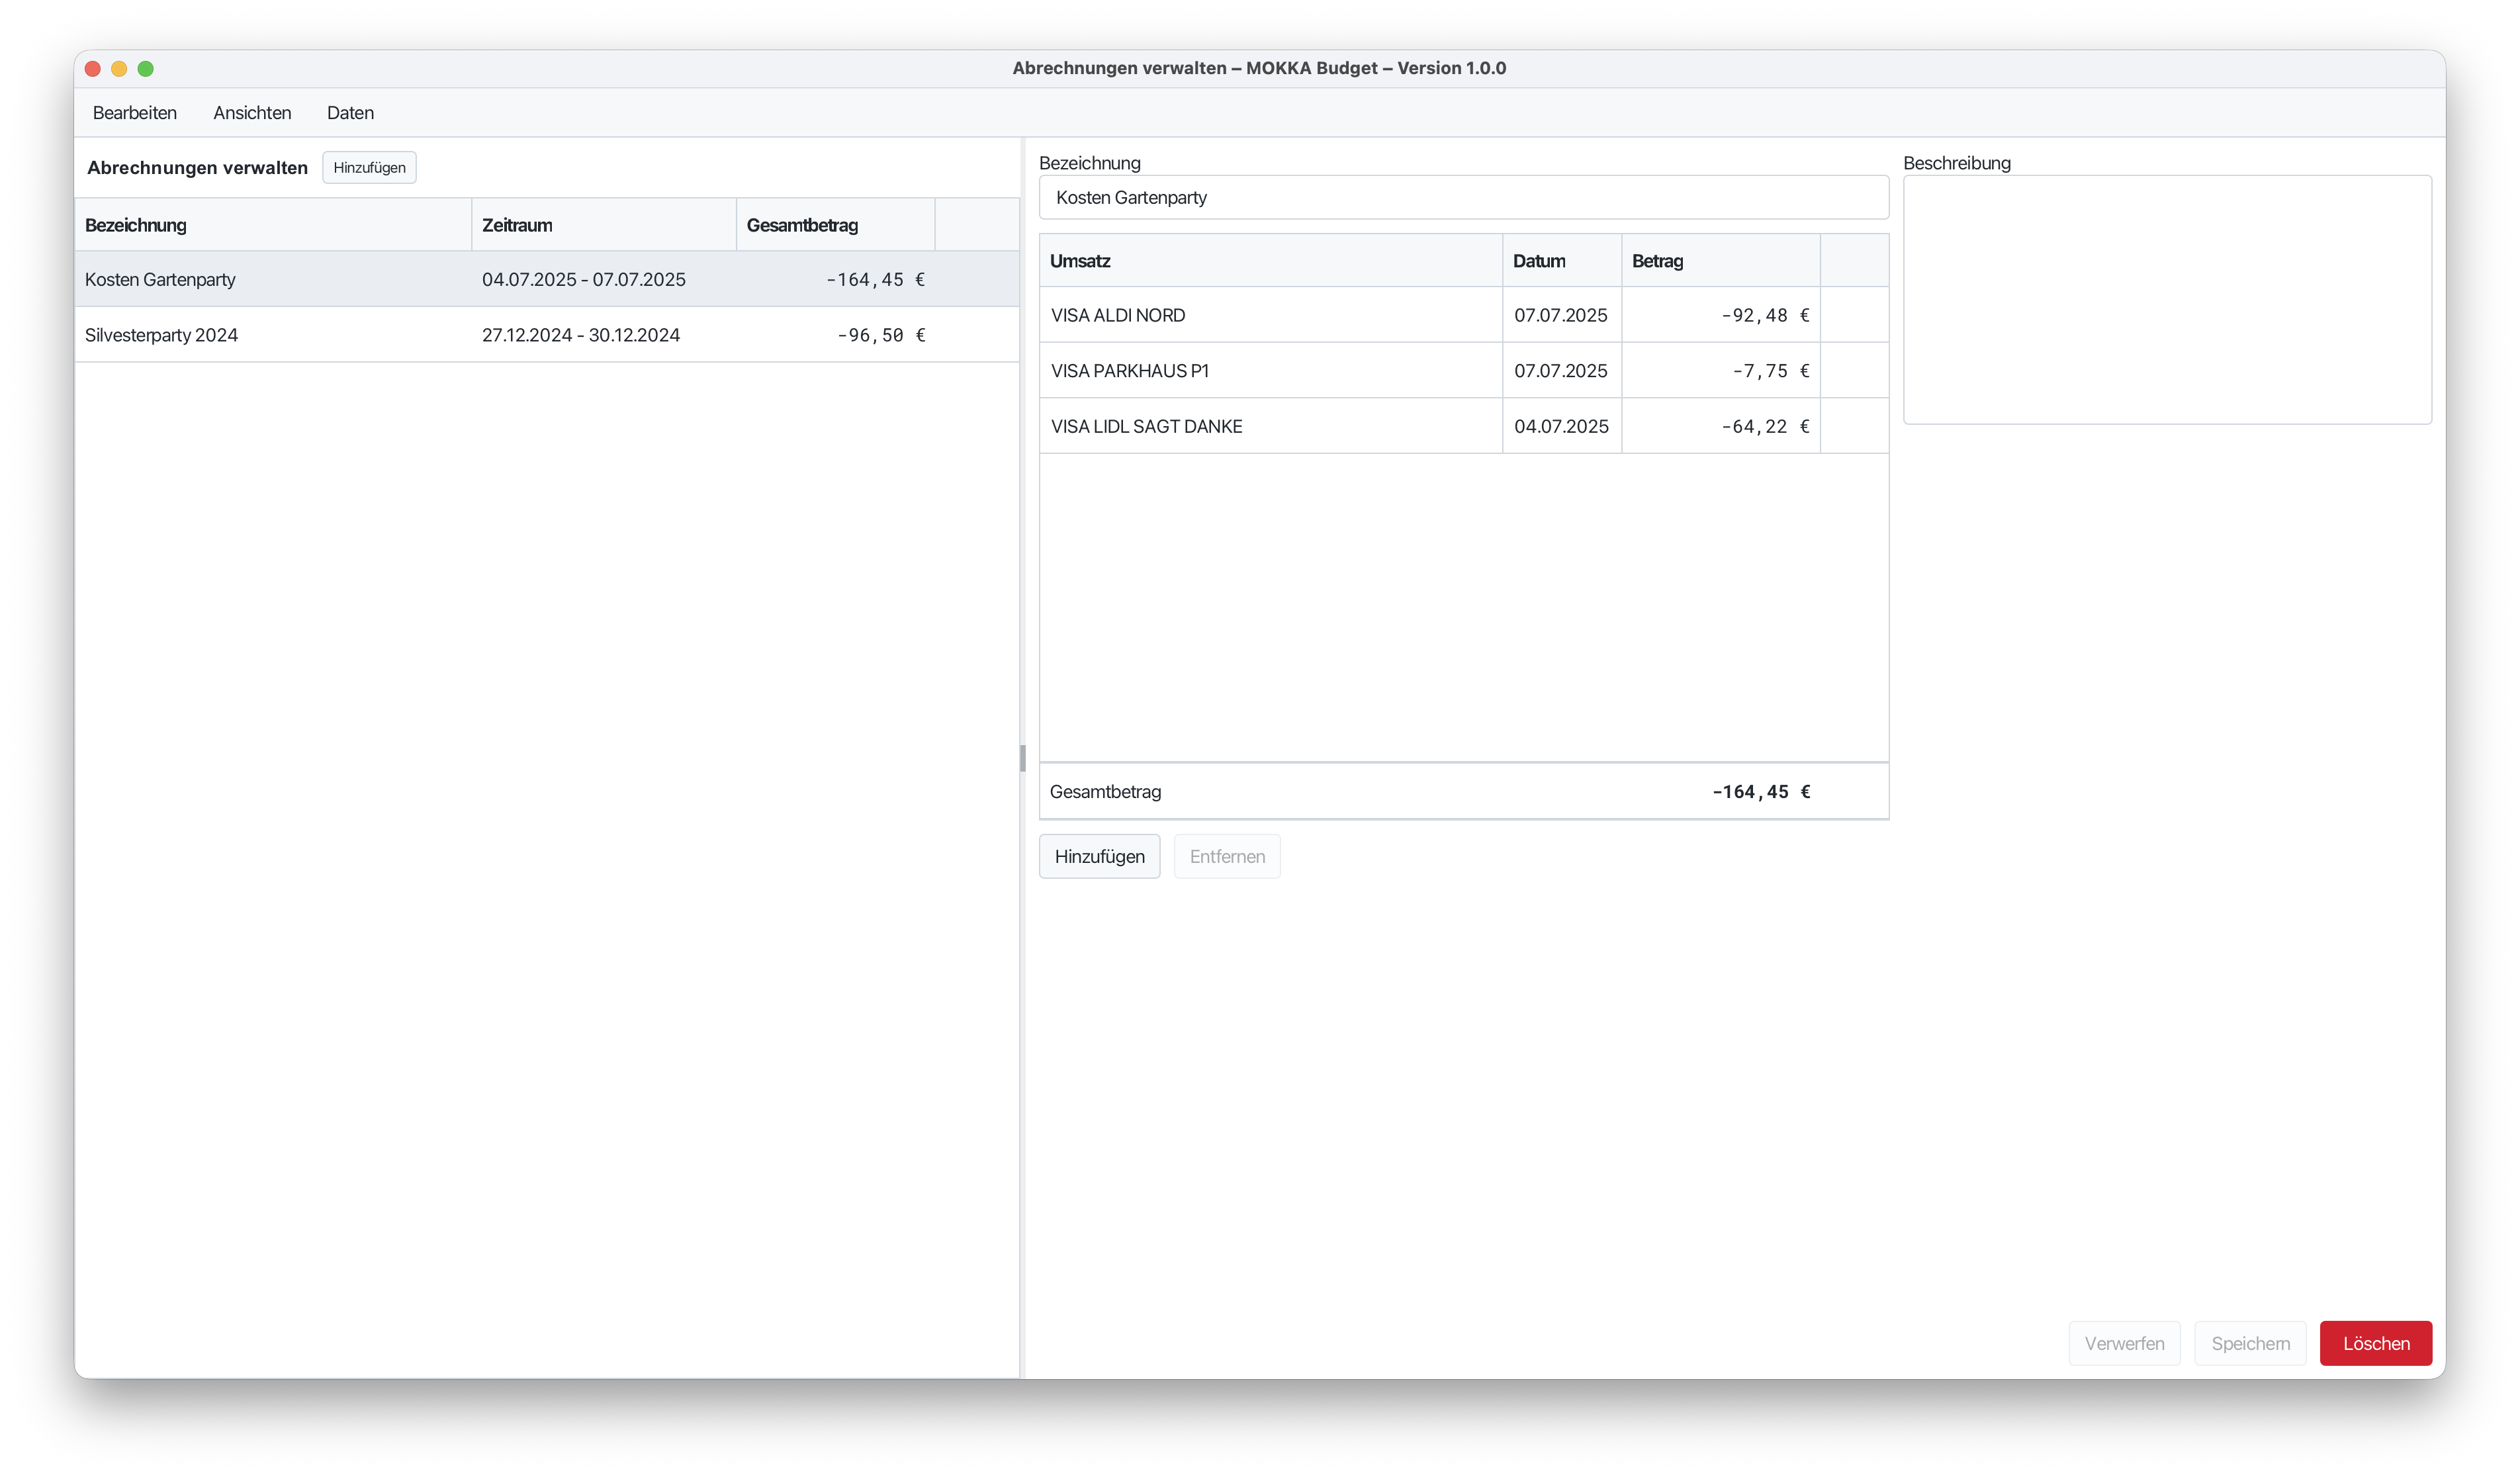
\includegraphics[width=\textwidth]{img/Screenshot-Billings-MDV}
	\vspace{-2em}
	\caption{Listen- \& Detailansicht der Abbrechnungen}
	\label{fig:mdvBillings}
\end{figure}

\section{Datenmodell} 

\begin{figure}[ht!]
	\centering
	\includegraphics[width=.8\textwidth]{img/DataModel}
	\vspace{0em}
	\caption{Datenmodell}
	\label{fig:datamodel}
\end{figure}

Datenmodel des Systems mit Stammdaten (grün und lila) sowie Bewegungsdaten (blau und grau).
\input{content/chap02}
\chapter{Ansichten}

Neben den Verwaltungsansichten, die eingehend erwähnt wurden, existieren drei Ansichten zur Auswertung der Ein- und Ausnahmen, die nachfolgend beschrieben werden.

\section{Monatsansicht}

Die Monatsansicht ermöglicht einen schnellen Überblick über alle Ausgaben eines Monats. Importierte Umsätze werden mit einem Icon gekennzeichnet, was somit anzeigt, dass eine Ausgabe bereits erfolgt ist. Das ist vor allem bei wiederkehrenden Ausgaben interessant, da dann der importierte Betrag in der Ansicht angezeigt wird -- gilt für alle Ansichten -- und nicht die geplante Ausgabe, wie sie im Tab "`Zahlungen"' in der Verwaltungsansicht der wiederkehrenden Ausgabe vorgemerkt ist (s. Abschnitt \ref{sec:fixedExpenses}).

\begin{figure}[ht!]
	\centering
	
\includegraphics[width=\textwidth]{img/Screenshot-MonthlyOverview}
	\vspace{-2em}
	\caption{Monatsansicht / Dashboard (aktueller Monat: August 2025)}
	\label{fig:MonthlyOverview}
\end{figure}

Neben der Tabelle auf der linken Seite, findet sich in der Mitte eine detailliertere Aufschlüsselung der Ausgaben pro Kategorie in dem angezeigten Monat.
Außerdem zeigt ein Diagramm die Entwicklung der Ausgaben in den letzten 12 Monaten an -- ausgehend von dem angezeigten Monat. So können Trends einfach erkannt werden.

Auf der rechten Seite werden alle aktiven Budgets mit deren Füllstand angezeigt. Sollte ein Budget zu 90\% oder mehr aufgebraucht sein, wird der Balken rot eingefärbt.


\section{Jahresansicht}

Die Jahresansicht ermöglicht die Übersicht aller wiederkehrenden Ausgaben eines Jahres -- gruppiert nach Kategorie (s. Abbildung \ref{fig:AnnualOverview}). Dabei ist die Ansicht in 2 Tabellen unterteilt:

Die obere Tabelle stellt die Ein- und Ausgaben eines jeden Monats gegenüber, sodass der Saldo pro Monat schnell abgelesen werden kann. Außerdem kann der oberen Tabelle unten rechts das Gesamtsaldo des betrachteten Jahres entnommen werden.

Während die Einnahmen nicht weiter aufgeschlüsselt werden, werden die wiederkehrenden Ausgaben gruppiert nach Kategorien in der unteren Tabelle detaillierter dargestellt. Eine Zelle enthält jeweils die Höhe einer wiederkehrenden Ausgabe pro Monat und ganz rechts in der Spalte "`Jahr"' die Gesamtsumme der Ausgabe (also bspw. wie viel Geld für Tanken fällig wurde). Alle anderen -- also einzigartige -- Ausgaben, die keinem wiederkehrenden Umsatz zugeordnet sind, werden pro Kategorie als "`Sonstige"' zusammengefasst.

\begin{figure}[ht!]
	\centering
	\includegraphics[width=\textwidth]{img/Screenshot-AnnualOverview}
	\vspace{-2em}
	\caption{Jahresansicht (aktueller Monat: August 2025)}
	\label{fig:AnnualOverview}
\end{figure}

\subsection*{Beispiel: Wocheneinkauf}

In Abbildung \ref{fig:AnnualOverview} kann erkannt werden, dass die geplanten Ausgaben für den Wocheneinkauf pro Monat überschritten werden. Ab August 2025 werden 350 Euro bis zum Ende des Jahres aufgeführt, das ist das Planungselement, welches bei dem wiederkehrenden Umsatz "`Wocheneinkauf"' unter "`Zahlungen"' hinterlegt ist (s. Abschnitt \ref{sec:fixedExpenses}). Hier könnte jetzt genauer in die Analyse gegangen werden, weshalb die Ausgaben höher als erwartet sind oder das Planungselement nach oben korrigiert werden. Dann würden bspw. 400 Euro in Zukunft geplant werden und bspw. im Jahr 2026 pro Monat für Wocheneinkäufe angezeigt werden. Somit kann Ende des Jahres bpsw. in das nächste Jahr geschaut werden, um herauszufinden, wie hoch die Fixkosten pro Monat voraussichtlich sein werden.

\textit{Anmerkung}: Es gibt aktuell keine Ansicht, die eine Auflistung aller Ausgaben (inkl. einzigartiger Ausgaben) pro Monat oder Jahr ermöglicht und dabei eine Summe bildet. Sollte eine solche Ansicht benötigt werden, kann etwas ähnliches über die Analyseansicht erreicht werden, indem eine Kategorie ausgewählt und im Diagramm auf den Balken des entsprechenden Monats geklickt wird. So kann -- etwas umständlich -- eine Aufschlüsselung aller Ausgaben eines Monats mit dazugehöriger Summe vorgenommen werden.

\section{Analyseansicht}

Die Analyseansicht ermöglicht die Untersuchung der Ausgaben einer Umsatzkategorie, um die Entwicklung der Ausgaben innerhalb eines gewählten Zeitraums nachvollziehen zu können. Die Visualisierung erfolgt mithilfe eines Balkendiagramms, welches drei Achsen hat: Eine Abszissenachse (x-Achse) und zwei Ordinatenachsen (y-Achsen). 

Die x-Achse zeigt die Monate und die linke y-Achse zeigt die Höhe der Ausgaben in dieser Kategorie für den jeweiligen Monat. Die rechte x-Achse zeigt die kumulierte Höhe der Ausgaben für den dargestellten Zeitraum. Diese Kumulation wird als Linie auf dem Balkendiagramm dargestellt.   

Sollte ein Budget für die ausgewählte Kategorie gepflegt sein, wird dieses als horizontale, rot gestrichelte Linie angezeigt. Diese Linie richtet sich in Abhängigkeit des eingestellten Budgettyps ("`monatlich"' oder "`jährlich"') entweder an der linken oder rechten Abszissenachse aus. 

Ein Klick auf einen Balken befüllt die Tabelle auf der rechten Seite der Ansicht und deckt somit alle Ausgaben des Monats innerhalb dieser Kategorie auf (s. Abbildung \ref{fig:AnalsisView}).

\begin{figure}[ht!]
	\centering
	\includegraphics[width=\textwidth]{img/Screenshot-AnalysisView}
	\vspace{-2em}
	\caption{Analyseansicht (geklickt auf den Balken "`November 2024"')}
	\label{fig:AnalsisView}
\end{figure}

\chapter{Datenbank-Verschlüsselung} \label{chap:dbEncryption}

Alle Anwendungsdaten werden lokal in einer SQLite-Datenbank gespeichert. Optional kann diese Datei mit einem Passwort verschlüsselt werden, sodass die Daten ohne Kenntnis des Passworts nicht lesbar sind.

\section{Erststart}

Beim ersten Start der Anwendung -- solange noch keine Datenbank existiert -- kann ein Passwort festgelegt werden. Alternativ lässt sich die Verschlüsselung vorerst überspringen (Button \textit{Daten nicht verschlüsseln}). Die Verschlüsselung kann später jederzeit nachträglich aktiviert werden.

\section{Anwendungsstart mit verschlüsselter Datenbank}

Ist die Datenbank verschlüsselt, muss bei jedem Start das Passwort eingegeben werden. Bei falschem Passwort kann die Anwendung nicht gestartet werden. Wird der Dialog ohne gültiges Passwort geschlossen, beendet sich die Anwendung.

\section{Verschlüsselung verwalten}

Die Verwaltung der Verschlüsselung ist im Menü unter \textit{Daten $\rightarrow$ Datenbank-Verschlüsselung} erreichbar. Dort wird angezeigt, ob die Verschlüsselung aktiv ist.

\begin{itemize}[nosep]
	\item \textbf{Verschlüsselung aktivieren:} Für eine bisher unverschlüsselte Datenbank kann ein Passwort vergeben werden.
	\item \textbf{Passwort ändern:} Bei aktiver Verschlüsselung kann das Passwort unter Angabe des aktuellen Passworts geändert werden.
	\item \textbf{Verschlüsselung deaktivieren:} Die Datenbank wird wieder unverschlüsselt gespeichert. Dies erfordert eine Bestätigung.
\end{itemize}

Vor dem Aktivieren oder Deaktivieren der Verschlüsselung erstellt die Anwendung automatisch eine Sicherungskopie der Datenbankdatei (Dateiendung \texttt{.backup.db} neben der eigentlichen Datenbankdatei).

\begin{infobox}
\textbf{Wichtig -- Passwortverlust}: Das Passwort wird nicht gespeichert und kann nicht zurückgesetzt werden. Geht das Passwort verloren, sind alle Anwendungsdaten unwiederbringlich verloren.
\end{infobox}

\begin{infobox}
\textbf{Hinweis bei Fehlern}: Schlägt das Aktivieren oder Deaktivieren der Verschlüsselung fehl, kann die Datenbank anhand der automatisch erstellten Sicherungskopie wiederhergestellt werden.
\end{infobox}



\end{document}
